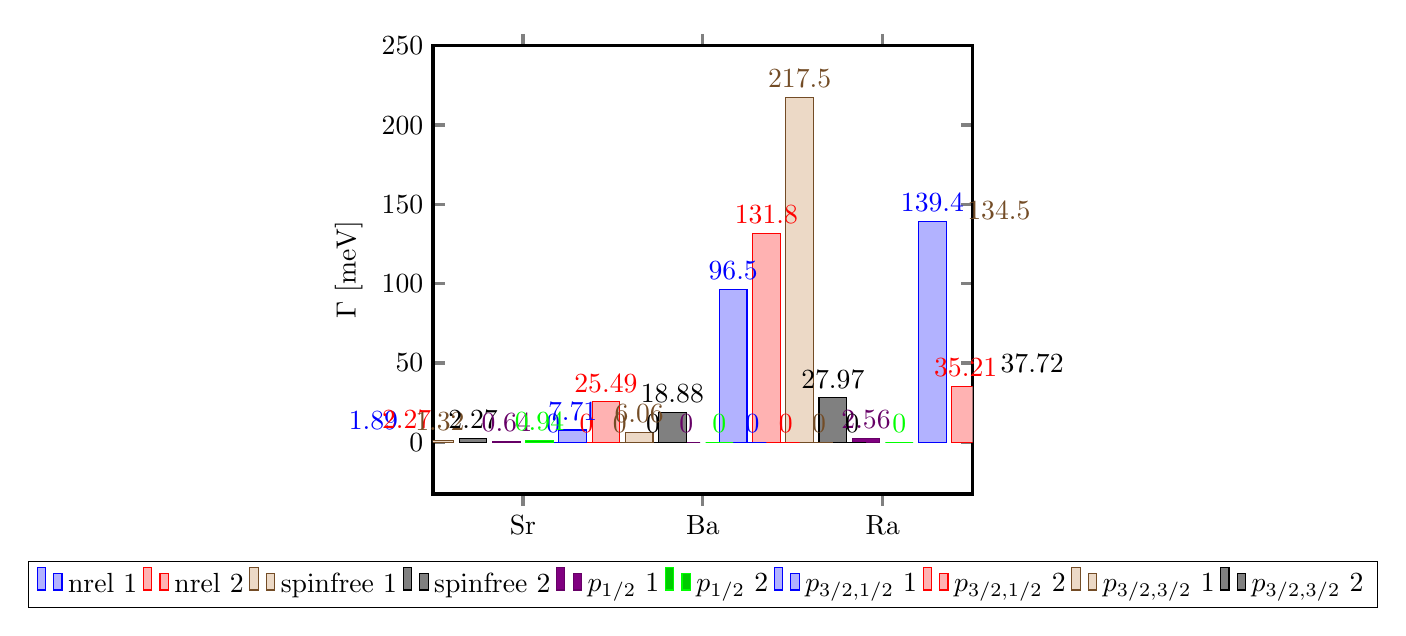
\begin{tikzpicture}
\begin{axis}[
    ybar,
    enlargelimits=0.15,
    legend style={at={(0.5,-0.15)},
      anchor=north,legend columns=-1},
    ylabel={$\Gamma$ [meV]},
    %ylabel={\#participants},
    symbolic x coords={Sr,Ba,Ra},
    xtick=data,
    nodes near coords,
    nodes near coords align={vertical},
    enlarge x limits=0.25, %space left and right
    axis line style = very thick,
    tick style = very thick
    ]
\addplot coordinates {(Sr,1.888) (Ba,0) (Ra,96.50)};
\addplot coordinates {(Sr,2.274) (Ba,0) (Ra,131.8)};
\addplot coordinates {(Sr,1.321) (Ba,0) (Ra,217.5)};
\addplot coordinates {(Sr,2.269) (Ba,0) (Ra,27.97)};
\addplot coordinates {(Sr,0.635) (Ba,0) (Ra,2.564)};
\addplot coordinates {(Sr,0.940) (Ba,0) (Ra,0)};
\addplot coordinates {(Sr,7.712) (Ba,0) (Ra,139.4)};
\addplot coordinates {(Sr,25.49) (Ba,0) (Ra,35.21)};
\addplot coordinates {(Sr,6.064) (Ba,0) (Ra,134.5)};
\addplot coordinates {(Sr,18.88) (Ba,0) (Ra,37.72)};
\legend{nrel 1,nrel 2,spinfree 1,spinfree 2,$p_{1/2}$ 1,$p_{1/2}$ 2,$p_{3/2,1/2}$ 1,$p_{3/2,1/2}$ 2,$p_{3/2,3/2}$ 1,$p_{3/2,3/2}$ 2};
\end{axis}
\end{tikzpicture}

